\chapter{Testes}
\label{chap:Plataformas}


\begin{figure}[htb]
	\caption{\label{fig:modulos-esp}Ambiente de teste}
	\begin{center}
		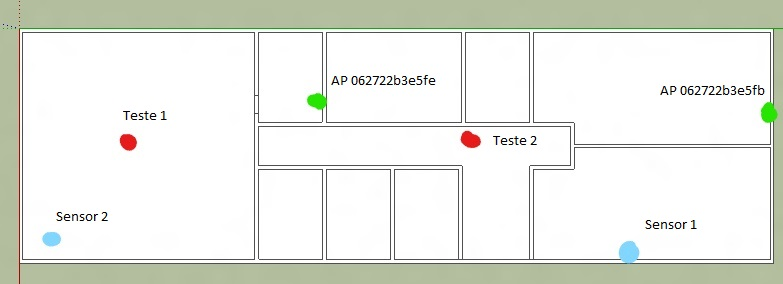
\includegraphics[width=1\textwidth]{060-testes/data-analisis/planta-baixa_Ink_LI.jpg}
	\end{center}
	\legend{Fonte: Elaborada pelo autor}
\end{figure}


Para entender  o ambiente onde a aplicação foi desenvolvida e testada no âmbito
de ruído wi-fi e pontos de referência wi-fi foi executada uma captura de teste
durante a noite quando ninguém habitava o prédio prototipo.

Nesta captura dois sensores foram utilizados posicionados a menos de 10 centímetros
de distância um do outro sobre uma mesa a um metro do chão a captura ocorreu de 2:50
até aproximadamente 11:25 totalizando aproximadamente 8 horas de captura

A captura foi executada com o comando


\begin{lstlisting}[language=bash]
tshark -I -i wlan0 -T fields -E header=y -E quote=d -e wlan.sa -e wlan.sa_resolved -e wlan.ta -e wlan.ta_resolved -e radiotap.dbm_antsignal -e wlan_mgt.ssid >> 2017-01-17--02-48--rpi-02.csv &
\end{lstlisting}

A análise de dados foi feita com a função \emph{summary} da ferramenta \emph{Ron’s editor}
e a filtragem com a função \emph{Filter} da ferramenta \emph{RecCsvEditor}

https://www.ronsplace.eu/Products/RonsEditor

http://recsveditor.sourceforge.net/

Para o primeiro sensor foram detidos 1 729 624 pacotes num arquivo de 155MB
com 88 transmissores únicos dos quais se destacaram dois endereços MAC que são os
pontos de acesso para rede wi-fi do laboratório.


\begin{figure}[htb]
	\caption{\label{fig:modulos-esp}Distribuição do dBm pelo tempo - 062722b3e5fb sensor 1}
	\begin{center}
		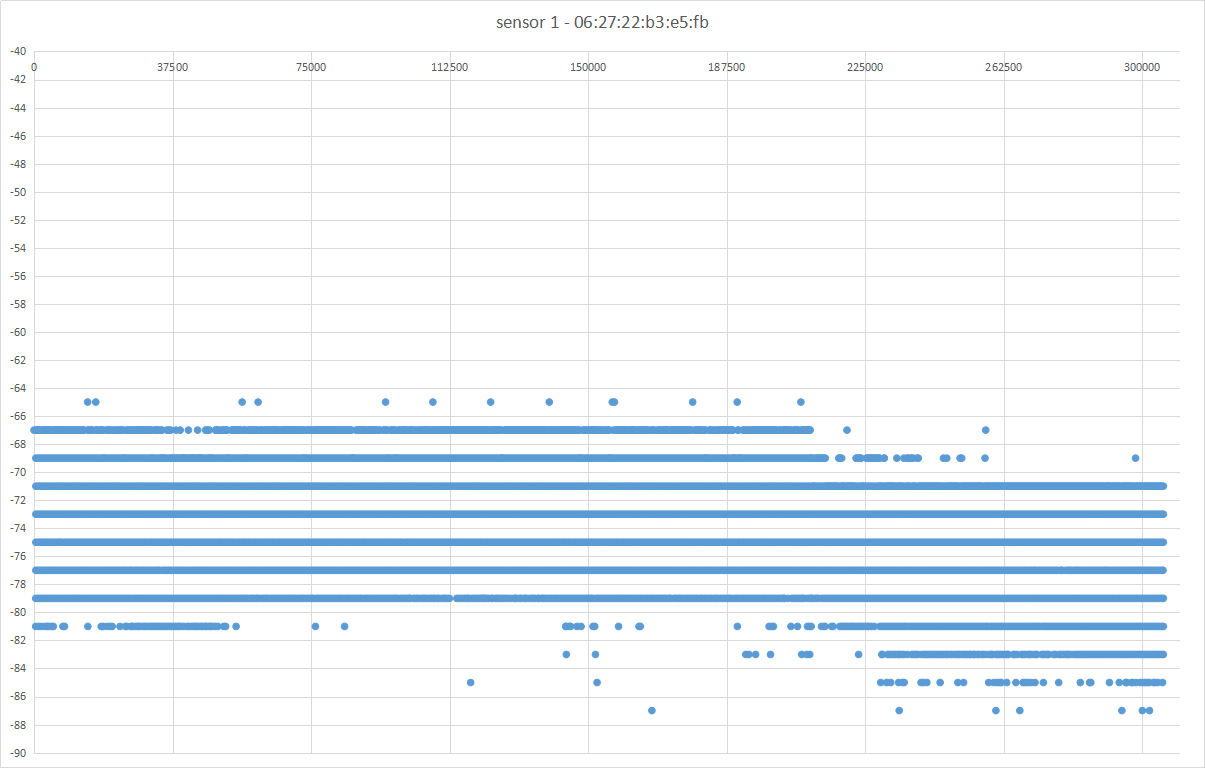
\includegraphics[width=1\textwidth]{060-testes/data-analisis/night-run/062722b3e5fb-sensor-01.png}
	\end{center}
	\legend{Fonte: Elaborada pelo autor}
\end{figure}

\begin{figure}[htb]
	\caption{\label{fig:modulos-esp}Distribuição do dBm pelo tempo - 062722b3e5fb sensor 2}
	\begin{center}
		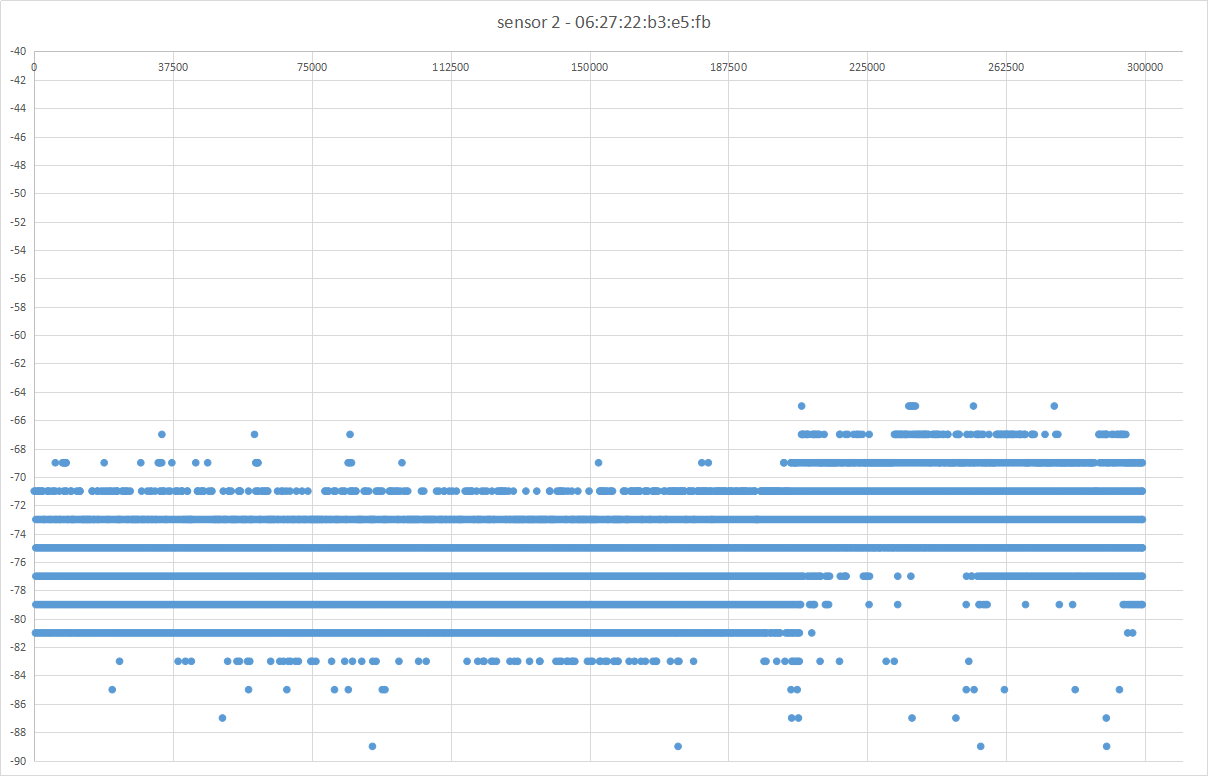
\includegraphics[width=1\textwidth]{060-testes/data-analisis/night-run/062722b3e5fb-sensor-02.png}
	\end{center}
	\legend{Fonte: Elaborada pelo autor}
\end{figure}

\begin{figure}[htb]
	\caption{\label{fig:modulos-esp}Distribuição do dBm pelo tempo - 062722b3e5fe sensor 1}
	\begin{center}
		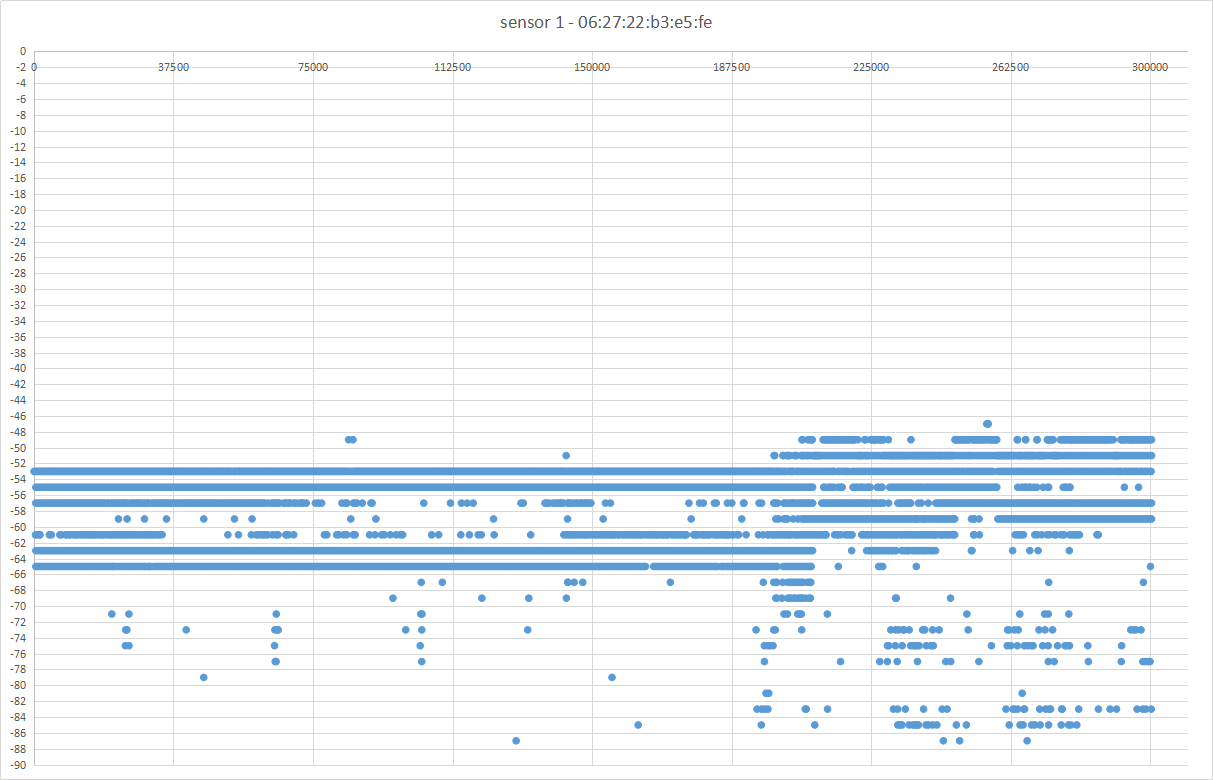
\includegraphics[width=1\textwidth]{060-testes/data-analisis/night-run/062722b3e5fe-sensor-01.png}
	\end{center}
	\legend{Fonte: Elaborada pelo autor}
\end{figure}

\begin{figure}[htb]
	\caption{\label{fig:modulos-esp}Distribuição do dBm pelo tempo - 062722b3e5fe sensor 2}
	\begin{center}
		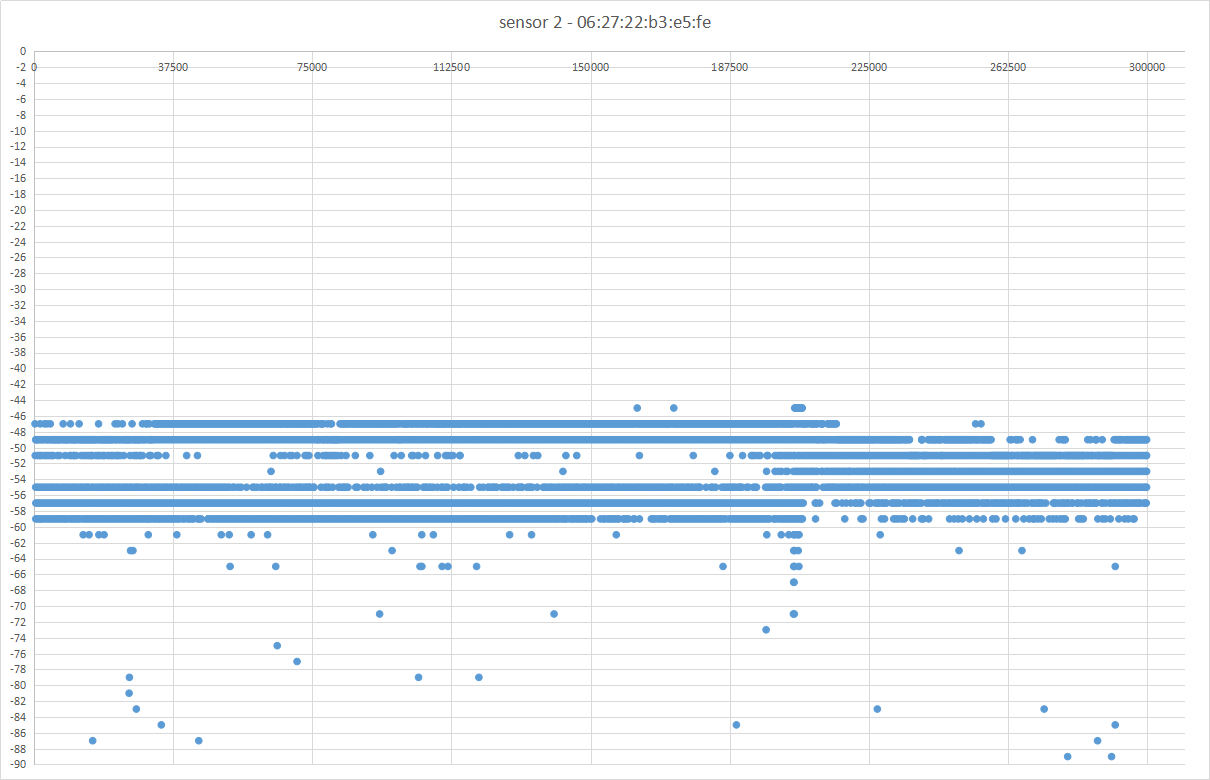
\includegraphics[width=1\textwidth]{060-testes/data-analisis/night-run/062722b3e5fe-sensor-02-.png}
	\end{center}
	\legend{Fonte: Elaborada pelo autor}
\end{figure}

\begin{figure}[htb]
	\caption{\label{fig:modulos-esp}dBm Pontos de acesso - Acumulado 8 horas}
	\begin{center}
		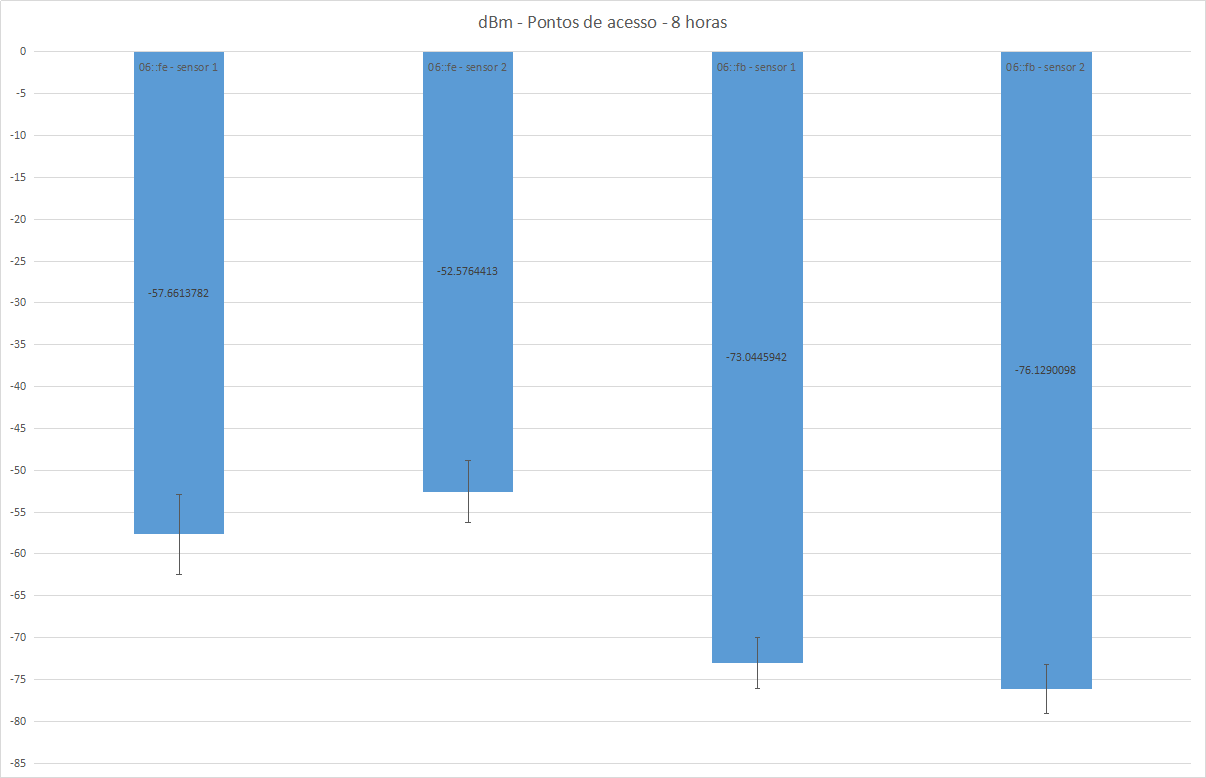
\includegraphics[width=1\textwidth]{060-testes/data-analisis/night-run/dBm-Pontos_de_acesso-8horas.png}
	\end{center}
	\legend{Fonte: Elaborada pelo autor}
\end{figure}


// Modo de uso do tshark na aplicação,utilizar na construção
Neste modo de uso os resultados são direcionadas para a saída padrão
(stdout)  do terminal e podem ser capturados por outro programa no formato
de valores separados por vírgula (csv).  os campos escolhidos para captura
são *wlan.sa*, *wlan.sa_resolved*, *wlan.ta*, *wlan.ta_resolved*, *radiotap.dbm_antsignal* e *wlan_mgt.ssid*

Teste relação de distância com smartphone como objetivo

Para verificar a capacidade do sensores de localizar contextualmente um dispositivo
móvel, smartphone, foi utilizado. Este foi posicionado em duas salas diferentes, Em
cada uma das salas foi executada uma captura de 10 minutos. Para que houvesse tráfego
na rede o dispositivo móvel foi configurado para receber um stream de vídeo no aplicativo Netflix.

A captura foi realizada utilizando a ferramenta TShark da mesma maneira que é utilizada no
aplicativo. A descrição deste modo de operação pode ser encontrada no capítulo de construção.

$
tshark -I -i wlan1 -T fields -E separator=, -E quote=d -e wlan.sa -e wlan.sa_resolved -e wlan.ta -e wlan.ta_resolved -e radiotap.dbm_antsignal -e wlan_mgt.ssid >> sensor-02-distance-test-01.csv
$

Para o primeiro caso o dispositivo estava na mesma sala do sensor número 2 que é a maior
sala do prédio com 12  metros de comprimento por 10 metros  De largura. neste caso foram
capturados 157736 pacotes totalizando 9.7 megabytes pelo sensor 1 21974 pacotes totalizando
1.9 megabytes de captura pelo sensor 2.

No segundo teste o dispositivo móvel estava posicionado no corredor fora da sala do sensor 1
e distante do sensor 2.  neste teste o sensor 1 capturou 103555 pacotes totalizando 6.4 megabytes
de captura e o sensor 2 capturou 22635 pacotes totalizando 2 megabytes de captura

 posteriormente os arquivos de captura foram analisados com a ferramenta *Ron’s Editor*  para que um sumário fosse construído.


\begin{figure}[htb]
	\caption{\label{fig:modulos-esp}Captura total (noise) - Teste 1}
	\begin{center}
		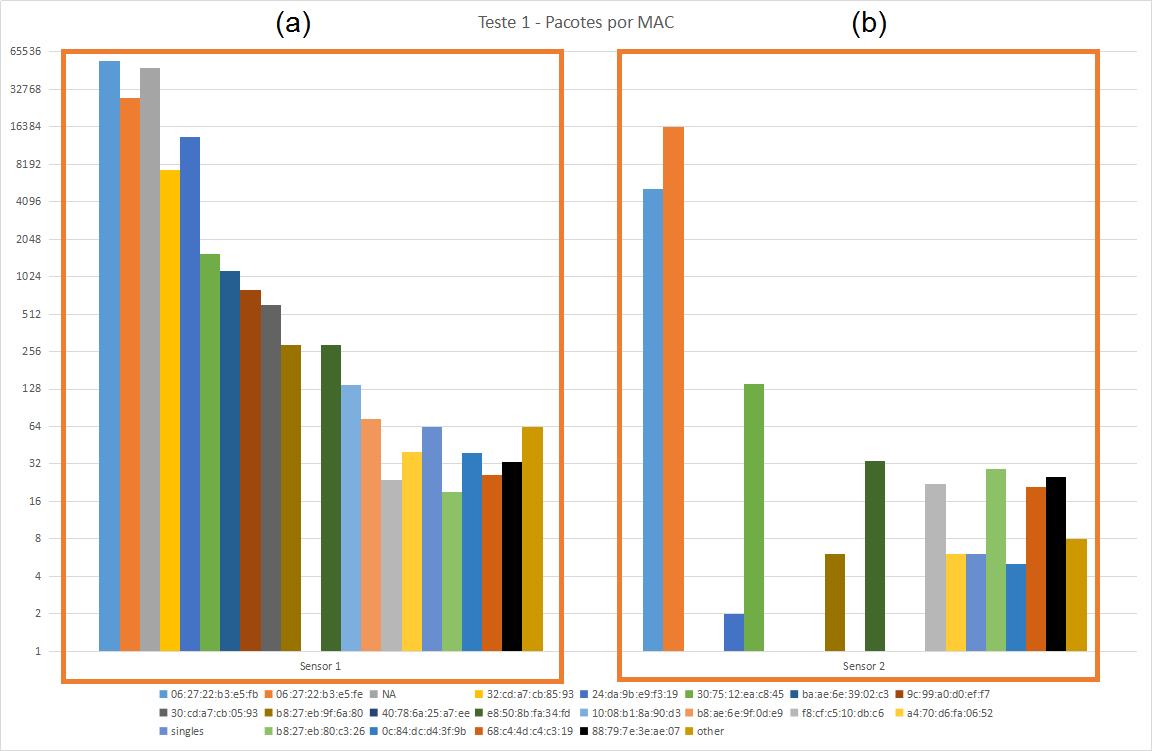
\includegraphics[width=1\textwidth]{060-testes/data-analisis/distance-mg4plus-netflix/Teste1.png}
	\end{center}
	\legend{Fonte: Elaborada pelo autor}
\end{figure}

\begin{figure}[htb]
	\caption{\label{fig:modulos-esp}Captura total (noise) - Teste 2}
	\begin{center}
		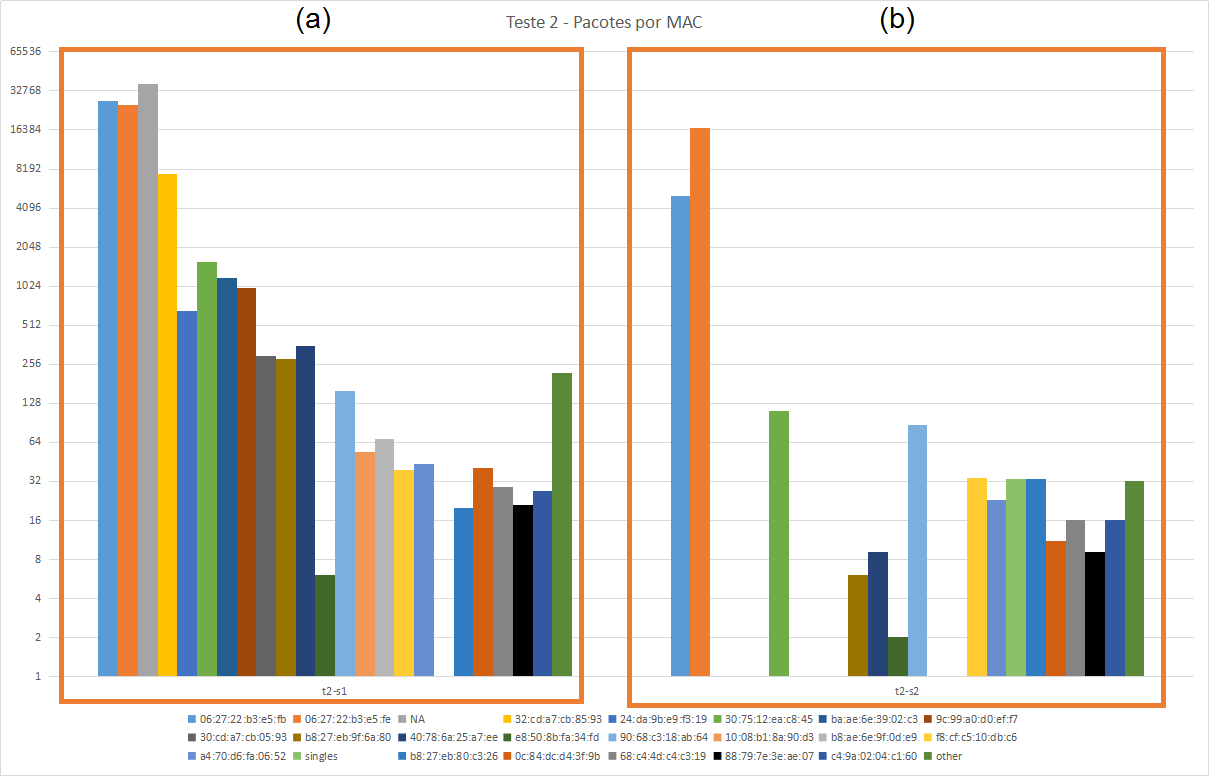
\includegraphics[width=1\textwidth]{060-testes/data-analisis/distance-mg4plus-netflix/Teste2.png}
	\end{center}
	\legend{Fonte: Elaborada pelo autor}
\end{figure}


\begin{figure}[htb]
	\caption{\label{fig:modulos-esp}dBm Motorola G4+ - Teste 1}
	\begin{center}
		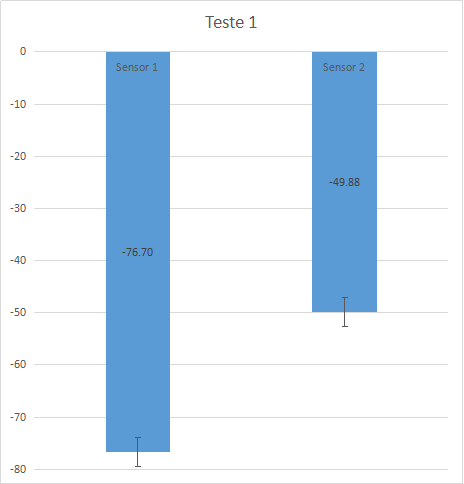
\includegraphics[width=1\textwidth]{060-testes/data-analisis/distance-mg4plus-netflix/target-Teste1.png}
	\end{center}
	\legend{Fonte: Elaborada pelo autor}
\end{figure}

\begin{figure}[htb]
	\caption{\label{fig:modulos-esp}dBm Motorola G4+ - Teste 2}
	\begin{center}
		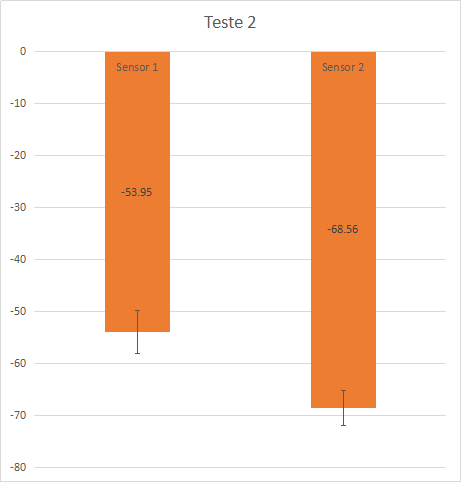
\includegraphics[width=1\textwidth]{060-testes/data-analisis/distance-mg4plus-netflix/target-Teste2.png}
	\end{center}
	\legend{Fonte: Elaborada pelo autor}
\end{figure}
